\section{校园网的具体实现}
\subsection{基本功能}%=============================================1
	\subsubsection{内网访问外网}
\indent  该项目中使用的Quidway R2621为具有NAT功能的路由器。我们采用NAT池的放那公式将内部IP映射到外部网络. 当有数据进行通信时,就按照一定的策略从地址池中选择一个公网IP地址进行转换,通信结束后,重新放入地址池中,这样如果有10个公网IP地址,可以同时令10台主机接入外网。\\
\indent  路由器的E1端的IP地址是192.168.137.2/24。E0端的IP地址是192.168.20.2/24。首先,在局域网内部的私有地址是不能访问外网的,数据包的源IP地址必须转换成公有地址才能在Internet上进行传输。学校内部网络在访问Internet上的服务器时,需要把IP地址进行转换。\\

\indent \textbf{路由器的设置步骤:} 
\begin{enumerate}
\item 设置外网的IP地址池 192.168.137.10/24——192.168.137.20/24;
\item 在路由器出口,将E1口与地址池绑定;
\item 测试连通性
\end{enumerate}

\indent \textbf{内部主机访问Internet上的服务器的工作过程:}
\begin{enumerate}
\item PCA的IP地址是192.168.20.1/24,向外网服务器发送请求时,目的地址是59.75.17.10/24;
\item 路由器收到数据包后,查找NAT表,然后将源IP地址192.168.20.1/24转换为地址池中的某个IP 192.168.137.x/24;
\item 数据经过网络传输,到达服务器,服务器对请求进行处理并作出回应,数据包的源地址为59.75.17.10/24,目的地址是192.168.137.x/24;
\item 数据到达路由器后,查找NAT表,然后把目的地址192.168.137.x/24修改为192.168.20.1/24;
\item 数据包经过网络传输到达目的主机PCA。
\end{enumerate}
注:本次模拟项目中,无外网IP可用。故采用如下办法,将一台主机连接WiFi,然后使用网络共享,该主机共享时分配的IP地址是192.168.137.0/24。所以将192.168.137.0网段模拟为外网IP,设置路由器出口为192.168.137.2/24。将学校申请的外网IP模拟为192.168.137.10/24——192.168.137.20/24。\\
\indent \textbf{核心代码:}
\begin{lstlisting}
%首先通过acl定义允许源地址属于任意网段的数据流做NAT转换
acl
rule permit 1 source any
%其次配置NAT地址池,设置用于转换的地址范围为192.168.20.10到192.168.20.20
nat address-group 192.168.20.10 192.168.20.20 255.255.255.0 1
%最后将地址池与上面配置的ACl进行关联,并在端口Ethernet0/1的出口方向上进行应用
interface Ethernet0/1
nat outbound 1 address-group 1
quit
\end{lstlisting}
\subsubsection{外网访问内网服务器}
为了能让公共网络的主机访问校园内部的服务器,如http服务器,这样可以让Internet上的主机访问校园官方主页。该功能可以通过路由器的NAT功能实现,将某一内部IP静态映射为学校申请的外部公共IP即可。
\\
\indent IP配置情况:
\\
\indent 在该项目中服务器IP为192.168.10.10/24
\\
\indent 映射的公共IP为192.168.137.21/24
\\
\indent 设置步骤:
\begin{enumerate}
\item 进入路由器E1
\item 将内网服务器IP192.168.20.10/24发布到公网192.168.137.21/24
\item 使用192.168.137.22/24的主机模拟公网主机访问192.168.137.21/24
\end{enumerate}

\indent 核心命令如下:
\begin{lstlisting}
interface Ethernet1
nat server global 192.168.137.21 inside 192.168.10.10
\end{lstlisting}
\subsection{安全方面}%=============================================2
	VLAN的出现,使得通过二层设备连接的复数终端之间的通信更为流畅和高效。它有效的弥补了二层设备无法隔离广播风暴的缺点,同时又能制造出复数个相互隔离的小范围通信区域,一定程度上形成了一个相对安全和私密的通信环境。所以在我们的组网工程安全计划中,VLAN的设置是一个关键的部分。
	\subsubsection{二层设备Vlan设置}%==============================2.1
	依照我们工程所计划的实现功能来看,在二层设备上,我们选择基于端口来划分VLAN,这样效率比较高。其过程只需定义VLAN并将相应的端口添加进去便可。以端口划分VLAN的原理也比较容易理解:(如图\ref{fig:safe_1}示)\\
\begin{figure}[thbp!]
\centering
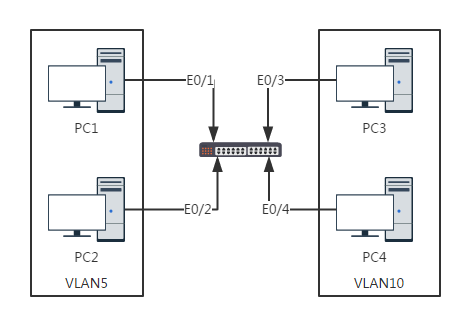
\includegraphics[width=0.7\linewidth]{figure/safe_1.png}
\caption{二层vlan示意图}
\label{fig:safe_1}
\end{figure}
\indent	端口E0/1和E0/2被划分在VLAN5中,则终端PC1与PC2处于一个虚拟网络中。PC1向PC2发送数据包时,数据包经过端口E0/1时会加上VLAN5的标签,然后在交换机中进行转发,到达E0/3、E0/4端口时发现这两个端口的VLAN编号与数据包标签编号不同,于是被丢掉;而到达E0/2端口时,发现编号相同,于是进行转发,在转发同时丢掉标签。\\
\indent	为了基于端口使用VLAN实现更复杂的功能,此处需简单说明Access,Trunk,以及Hybrid三个端口的区别。首先知道的是Access只允许单Vlan通过,而Trunk和Hybrid端口允许多Vlan通过。在这里我们从端口收报文(进入交换机方向)和端口发报文(送出交换机方向)两个方面来简单对比:\textbf{收报文时},三个端口均先检查该报文是否有VLAN标签,没有则均打上该端口的标签(tagged)并进行转发,有的话Access端口直接丢包,Trunk与Hybrid端口会判断该端口是否允许此VLAN的数据进入,允许则转发,不允许则丢弃。\textbf{发报文时},Access端口和Trunk端口会比较该端口VLANID与报文标签是否一致,一致则剥离(untagged)标签然后发送,不一致Access端口丢包,Trunk端口直接发送;Hybrid端口会先判断该报文标签Vlan在本端口的属性,若是untag则剥离标签发送,若是tag则保留标签发送。\\
\indent	我们所要设计的工程出发,如下图\ref{fig:safe_2}:图中S2,S3代表二层,三层交换机\\
\begin{figure}[thbp!]
\centering
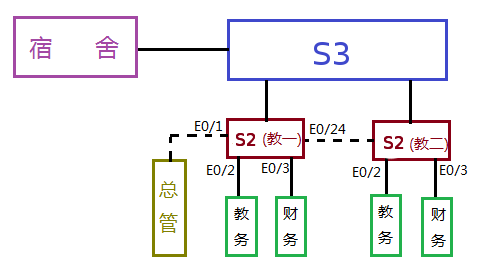
\includegraphics[width=0.7\linewidth]{figure/safe_2.png}
\caption{Vlan拓扑图说明}
\label{fig:safe_2}
\end{figure}
\indent	这里我们可以在二层设备间模拟出两种工作环境:\\
\indent 第一种:教一的总管可以与教务和财务互访,但教务和财务互相隔离。定义E0/1、E0/2、E0/3口Vlan分别为Vlan10、Vlan20和Vlan30,并将三个接口全设置为Hybrid。E0/1口设置Vlan10、20、30的报文不打标签(untagged)发送;E0/2口设置Vlan10、20不打标签发送;E0/3口设置Vlan10、30不打标签发送。这样便可实现第一种结构。代码如下:\\
\begin{lstlisting}
[Quidway]vlan 10
[Quidway - vlan10]port ethernet0/1
[Quidway - vlan10]quit
[Quidway]vlan 20
[Quidway - vlan20]port ethernet0/2
[Quidway - vlan20]quit
[Quidway]vlan 30
[Quidway - vlan30]port ethernet0/3
[Quidway - vlan30]quit

[Quidway]interface ethernet0/1
[Quidway - ethernet0/1]port link-type hybrid
[Quidway - ethernet0/1]port hybrid vlan 10 20 30 untagged
[Quidway - ethernet0/1]quit
[Quidway]interface ethernet0/2
[Quidway - ethernet0/2]port link-type hybrid
[Quidway - ethernet0/2]port hybrid vlan 10 20 untagged
[Quidway - ethernet0/2]quit
[Quidway]interface ethernet0/3
[Quidway - ethernet0/3]port link-type hybrid
[Quidway - ethernet0/3]port hybrid vlan 10 30 untagged
[Quidway - ethernet0/3]quit
\end{lstlisting}

\indent 第二种:教一教二的教务之间可以互通、财务之间可以互通,但教务和财务之间隔离。配置两个交换机的E0/2、E0/3口Vlan分别为Vlan20和Vlan30,配置两个交换机的E0/24接口为Trunk并允许所有Vlan通过。这样便能实现第二种结构。代码如下:\\
\begin{lstlisting}

%在“教一”“教二”上均进行如下配置:
[Quidway]vlan 20
[Quidway - vlan20]port ethernet0/2
[Quidway - vlan20]quit
[Quidway]vlan 30
[Quidway - vlan30]port ethernet0/3
[Quidway - vlan30]quit

[Quidway]interface ethernet0/24
[Quidway - ethernet0/24]port link-type trunk
[Quidway - ethernet0/24]port trunk permit vlan all
[Quidway - ethernet0/24]quit



\end{lstlisting}


	
	\subsubsection{三层设备Vlan设置以及ACL}%==================================================2.2
\indent	在三层交换机上设置Vlan,首先也是需要定义Vlan,然后为Vlan分配端口,最后进入Vlan视图里为此Vlan分配IP。由于我们使用的三层交换机已经默认启用了路由功能,设置好Vlan后经测试我们发现,Vlan间直接是互通的,路由表自动生成了。于是我们打算在此基础上进行一些安全方面的设计,其中需要用到ACL。\\
\indent	ACL,译为访问控制列表(Access Control List) 是路由器和交换机接口的指令列表,通过设定相应规则来控制端口进出的数据包。通过ACL理论上可以实现接口间的单向通信,从而扩展为三层Vlan间的单向通信。ACL具体作用流程如图\ref{fig:safe_3}:\\
\begin{figure}[thbp!]
\centering
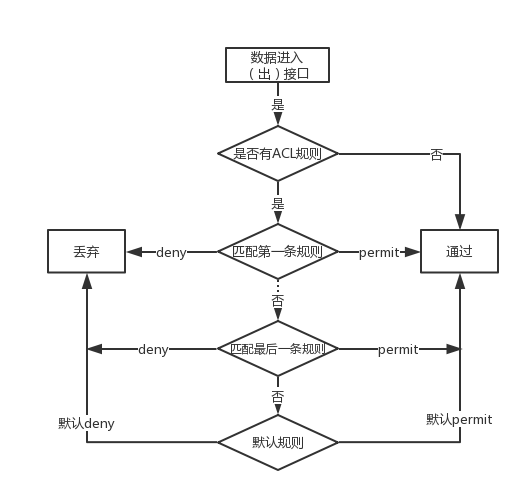
\includegraphics[width=0.7\linewidth]{figure/safe_3.png}
\caption{ACL流程图}
\label{fig:safe_3}
\end{figure}
\indent 在我们所拿到的三层交换机上进行实际ACL配置时,我们需要用到QOS(Quality of Service)策略。QOS指一个网络能够利用各种基础技术,为指定的网络通信提供更好的服务能力, 是网络的一种安全机制,是用来解决网络延迟和阻塞等问题的一种技术。配置QOS策略需要包含三个要素:流分类(traffic classifier),流行为(traffic behavior)和QOS策略(QOS policy)。具体流程如下:\\
\begin{enumerate}
\item 进入ACL访问控制列表视图并定义访问规则
\item 定义流分类
\item 定义流行为,确定符合流分类的报文并加以限制
\item 定义Qos策略,将流分类和流行为进行关联
\item 将QOS策略应用到相应端口
\end{enumerate}

\indent 代码如下:
\begin{lstlisting}
[H3C]vlan 10
[H3C - vlan10]port ethernet1/0/1
[H3C - vlan10]quit
[H3C]vlan 20
[H3C - vlan20]port ethernet1/0/2
[H3C - vlan20]quit

[H3C]interface vlan 10
[H3C-Vlan-interface10]ip address 192.168.10.1 24
[H3C-Vlan-interface10]quit
[H3C]interface vlan 20
[H3C-Vlan-interface20]ip address 192.168.20.1 24
[H3C-Vlan-interface20]quit

[H3C]acl number 3000
[H3C-acl-adv-3000]rule 1 deny ip source 192.168.10.0  0.0.0.255 destination 192.168.20.0 0.0.0.255
[H3C-acl-adv-3000]quit

[H3C]traffic classifier abc
[H3C-classifier-abc]if-match acl 3000
[H3C-classifier-abc]quit

[H3C]traffic behavior abc
[H3C-behavior-abc]filter deny
[H3C-behavior-abc]quit

[H3C]qos policy abc
[H3C-qospolicy-abc]classifier abc behavior abc
[H3C-qospolicy-abc]quit

[H3C]interface eth1/0/1
[H3C-Ethernet1/0/1]qos apply policy abc inbound
\end{lstlisting}

\begin{figure}[thbp!]
\centering
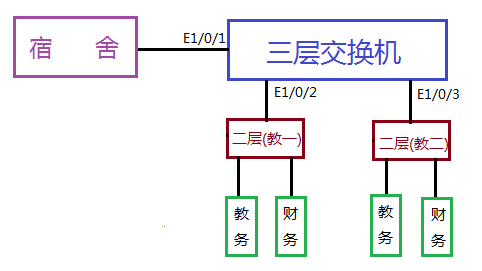
\includegraphics[width=0.7\linewidth]{figure/safe_4.png}
\caption{}
\label{fig:safe_4}
\end{figure}
\indent 由图\ref{fig:safe_4}说明,我们设定E1/0/1接口为Vlan10,IP段:192.168.10.0;\\
E1/0/2接口为Vlan20,IP段:192.168.20.0。若我们想要“宿舍”不能单向访问“教一”,则在E1/0/1接口Inbound方向设置ACL规则:禁止192.168.10.0到达192.168.20.0。这样的效果便是“教一”端可以访问“宿舍”,而反之不能。\\
\indent 但实际上我们在设置中出现了一个问题,经过反复思考和尝试还是不知道如何解决。利用刚才的例子来说明问题:我们在设置好“宿舍”不能单向访问“教一”之后,经过ping测试发现,从“宿舍”终端无法ping通“教一”的网关,自然也无法ping通其下终端,这一点和设计初衷吻合;从“教一”终端虽然能ping通“宿舍”网关,但无法ping通其下的终端。经检查也不是终端防火­墙的问题。该问题还需要进一步思考与查证。\\
\subsection{IP分配}%==================================================3
本着节约资源的角度, 应该给终端动态分配ip地址, 但是服务器应当是静态分配的.我们现在的方案是设置全局动态分配,但是把服务器的ip地址给剔除.\\
\indent DHCP(Dynamic Host Configuration Protocol,动态主机配置协议),即动态分配,当DHCP客户端第一次从DHCP服务器端租用到IP地址之后,并非永久地使用该地址,只要租约到期,客户端就得释放这个IP地址,以给其他工作站使用。在该校园网项目搭建过程中我们采用这种动态IP分配的方式,以避免主机IP地址错误或冲突的问题。
\\
\indent DHCP Client可以设置在三层交换机,路由器,或者服务器上。在这次项目中考虑到服务器的性能,并且与三层交换机的vlan功能相结合,我们将DHCP Client设置在三层交换机上。除了为普通主机动态分配IP,我们还为服务器设置了固定IP,这样可以为其它主机访问内网服务器提供便利。
\\
三层交换机DHCP与vlan划分情况:
\begin{enumerate}
\item vlan2
vlan interface 192.168.10.1/24
在此vlan中为服务器设置固定IP192.168.10.10/24
\indent vlan3
vlan interface 192.168.11.1/24
\indent vlan4
vlan interface 192.168.12.1/24
\indent vlan5
vlan interface 192.168.13.1/24
\indent vlan15
vlan interface 192.168.20.1/24
该vlan用来连接路由器
\end{enumerate}
路由器IP为192.168.20.2/24
\begin{enumerate}
\item 定义Vlan,并为此Vlan加入端口。
\item 进入Vlan视图,为此Vlan配置IP地址
\item 开启DHCP功能
\item 创建DHCP地址池并进入DHCP地址池视图
\item 为地址池设定动态分配IP的地址范围
\item 配置网关地址并将网关地址从地址池去除
(若要分配固定IP,将此IP从IP池中剔除即可)
\end{enumerate}
\subsection{服务器}%==================================================4
	该方案中的所有服务均集成在一台linux电脑上.
	\subsubsection{http服务}%========================================4.1
	首先开启http服务,该方案中用的是apach 
		\begin{lstlisting}[language=bash]
	$apt-get install apach2
	$/etc/init.d/apach2 start
	$nmap localhost
\end{lstlisting}
\begin{figure}[thbp!]
\centering
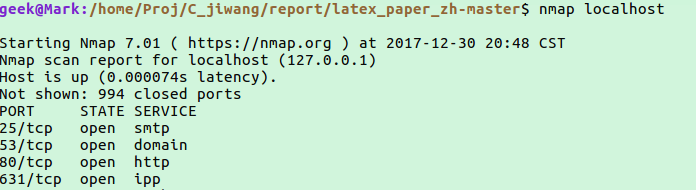
\includegraphics[width=0.9\linewidth]{figure/linux_http_start.png}
\caption{ 开启http服务}
\label{fig:linux_http_start}
\end{figure}

	\indent	图\ref{fig:linux_http_start}显示已开启http.为了查询linux服务器的ip, 需要执行:
		\begin{lstlisting}[language=bash]
	$ ifconfig
		\end{lstlisting}

\indent	把对应的html网页放在开启服务器的/var/www/http中后在其他终端的浏览器中输入对应的url就可以访问该网页,如图\ref{fig:linux_http_test} 所示.
		\begin{figure}[thbp!]
\centering

\includegraphics[width=0.9\linewidth]{figure/linux_http_test.png}
\caption{ 测试http服务}
\label{fig:linux_http_test}
\end{figure}
	\subsubsection{ftp服务}%===========================================4.2
	校园中资源共享很重要, 在此我们选择server/client的模式,选用ftp(File Transport Protocol).用户可以在服务器上进行上传和下载.\\
\indent	在linux主机上新建一个名为jiwang的用户, 将该用户的工作空间设为ftp根目录, 该设计采用vsftp来开启ftp服务.打开终端执行下列指令
	\begin{lstlisting}[language=bash]
	$ adduser jiwang	#创建用户,更具提示设置密码等信息
	$ apt-get install vsftpd 	#安装vsftpd
	$ service vsftpd start  #开启ftp服务	
	$ nmap localhost
	
	\end{lstlisting}

\begin{figure}[thbp!]
\centering
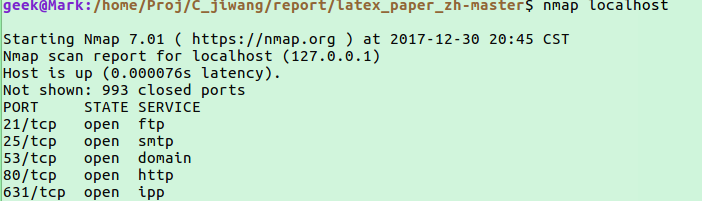
\includegraphics[width=0.9\linewidth]{figure/linux_ftp_start.png}
\caption{ 开启ftp服务}
\label{fig:linux_ftp_start}
\end{figure}
	
\indent	图\ref{fig:linux_ftp_start}	中显示已经开启ftp服务.相关的配置文件在/etc/vsftpd.confg中, 在里面可以设置用户的权限等信息.\\
\indent 找一台终端打开我的电脑, 输入对应的url,用户名,密码既可适用ftp服务,如图\ref{fig:linux_ftp_test}所示.
	\begin{figure}[thbp!]
\centering
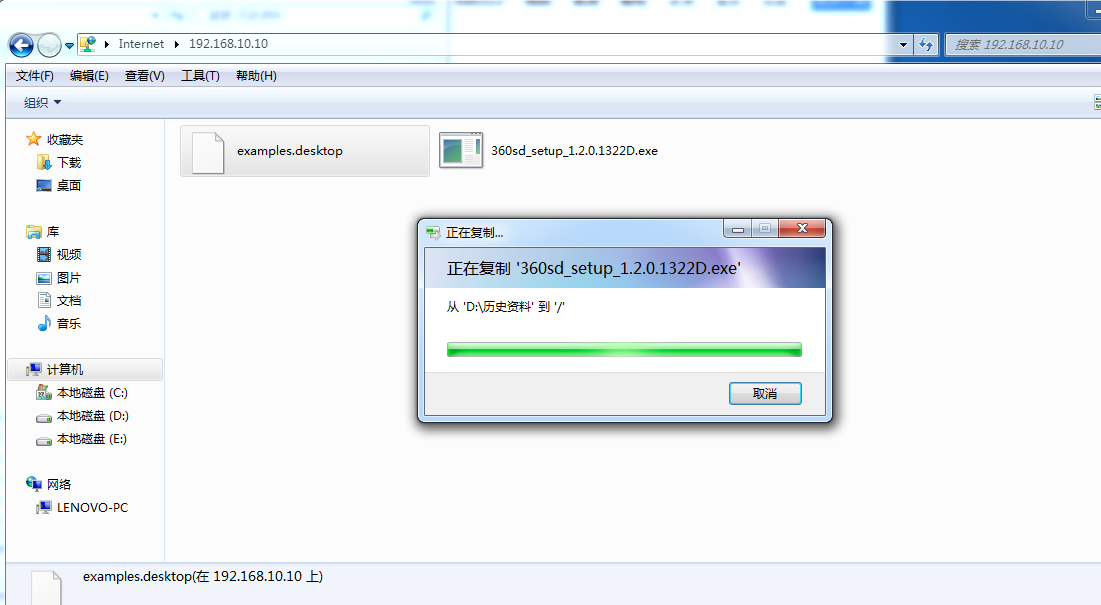
\includegraphics[width=0.9\linewidth]{figure/linux_ftp_test.png}
\caption{ 测试ftp服务}
\label{fig:linux_ftp_test}
\end{figure}
	\subsubsection{DNS服务}
	DNS(Domain Name System)本质上是一个域名和ip地址的映射表, 公网又公网的dns,如谷歌的8.8.8.8.我们要做一个内网dns, 这样不同终端访问的时候只需输入好记的域名既可.
	配置方法为:
\begin{lstlisting}[language=bash]
	$ apt-get install dnsmasq
\end{lstlisting}

\indent	相关的配置在/etc/dnsmasp.conf中, 里面可以将内网的ip的域名进行映射,如图\ref{fig:linux_dns_conf}\\
\begin{figure}[thbp!]
\centering
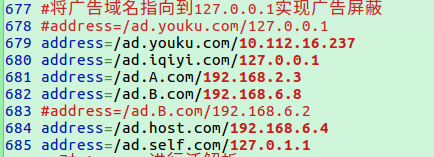
\includegraphics[width=0.9\linewidth]{figure/linux_dns_conf.png}
\caption{配置dns}
\label{fig:linux_dns_conf}
\end{figure}
	通过ping对应的域名来见测dns是否生效,如图\ref{fig:linux_dns_test}所示
\begin{figure}[thbp!]
\centering
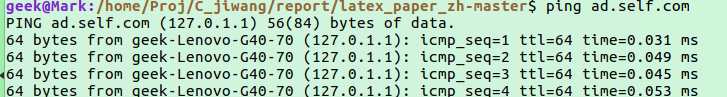
\includegraphics[width=0.9\linewidth]{figure/linux_dns_test.png}
\caption{配置dns}
\label{fig:linux_dns_test}
\end{figure}

\indent	目前的测试结果是, 只有和服务器在同一个3层vlan中的终端才能够使用dns服务, 猜测是我们在3层交换机的配置中有所遗漏.因为一开始dns服务是可以跨vlan的, 后面对3层交换机进行许多配置后就不可以了.
